%% main.tex --- Computers & Security submission (elsarticle)
%% W7.3 submission fixes: no manual section numbers, figures/tables placed in the body,
%% declarations in the manuscript, one notation for criteria and gates, US spelling.
\documentclass[preprint,12pt]{elsarticle}
\usepackage[T1]{fontenc}
\usepackage{cmap}  % T1 字体的 ToUnicode：破折号、引号、连字可正确抽取
\usepackage{lmodern}
\usepackage{graphicx,booktabs,amsmath,amssymb,amsthm}
\usepackage[colorlinks=true,linkcolor=blue,citecolor=blue,urlcolor=blue]{hyperref}
\graphicspath{{figures/}}
\journal{Computers \& Security}

\hypersetup{
  pdftitle={The feasible region of cross-call aggregation exfiltration on LLM agents: why coverage-closure criteria cannot buy low misfire and high residual uncertainty},
  pdfauthor={Peiyuan Li},
  pdfkeywords={LLM agent; tool calling; data exfiltration; aggregation; coverage closure; measurement},
  pdfsubject={Computers \& Security}
}

\renewcommand{\floatpagefraction}{0.85}  % 只让接近满页的浮动页成立，否则优先页顶＋正文
\renewcommand{\topfraction}{0.85}
\renewcommand{\bottomfraction}{0.7}
\setcounter{topnumber}{2}
\setcounter{bottomnumber}{2}
\setcounter{totalnumber}{3}

\hyphenation{AgentRaft MAScope}
\newtheorem{theorem}{Theorem}
\newtheorem{proposition}{Proposition}
\newtheorem{lemma}{Lemma}

\begin{document}
\begin{frontmatter}
\title{The feasible region of cross-call aggregation exfiltration on LLM agents:
why coverage-closure criteria cannot buy low misfire and high residual uncertainty}
\author{Peiyuan Li\corref{cor1}\fnref{fn1}}
\ead{202483280093@nuist.edu.cn}

\cortext[cor1]{Corresponding author}
\address{School of Cyber Science and Engineering, Nanjing University of Information
Science and Technology, Nanjing 210044, China}
\fntext[fn1]{ORCID: 0009-0008-7982-9597}
\begin{abstract}
The exfiltration we care about is aggregation-based: the agent moves a secret out fragment by
fragment, where every individual call is legitimate. For the single-field coverage-closure family
the result is an empty feasible region under four checkable assumptions (H1--H4): the 24-bit
uncertainty gate (5) forces $\theta' \leq 7/12$, the 30\% benign-cost gate (1) forces
$\theta' \geq \theta^{*} > 7/12$, and no $\theta'$ satisfies both. Under H3 the
post-interception nominal remaining uncertainty is $R = 4\cdot(L-\text{delivered}) \geq
4L(1-\theta') + 4 - 4\delta_{\mathrm{rem}}$ ($\delta_{\mathrm{rem}}$ the ceiling remainder), safely
$R \geq 4L(1-\theta')$;
at $\theta' = 1.0$ this gives $R = 4$ bit with $H = 0.975$. The correct statement is therefore
conditional on the workload: the empty region is write-granularity-independent and determined by
the per-task final-coverage distribution. The 234-combination scan (102 combinations in the
candidate pool) instantiates the proposition and is not part of its proof: under the union and
unique ambiguity readings the scan yields 0/102 combinations passing all five gates (Wilson 95\%
upper bound 3.6\%). On the second workload the picture is direction-consistent but power-limited:
airline field-level write tasks, $n = 15$ --- quantitatively this paper is anchored to retail, and
no workload-independence is claimed.
\end{abstract}
\begin{keyword}
LLM agent \sep tool calling \sep data exfiltration \sep aggregation \sep coverage closure \sep measurement
\end{keyword}
\end{frontmatter}

\section{Introduction}\label{sec:intro}

A tool-using language-model agent acts through calls. Each call declares what it reads or writes,
and each is authorized on its own. A secret held in a registered field can leave through such calls
without any single one of them being a violation: the agent copies a few bytes per call into a tool
argument, the tool writes them to a sink the user is entitled to use, and the secret is reassembled
outside. Nothing in one call is anomalous --- the lengths are plausible, the destination is
permitted, and the content is a substring of a field the agent may read. The violation exists only
in the assembly, and the assembly is in no single call's transcript. Per-call inspection is
therefore structurally blind to the threat, and any remedy has to carry state across calls.

This paper asks what such state can buy, and at what price. Three readings have to be reported
together for an answer to mean anything: whether the criterion can tell a dangerous trace from a
benign trace of the same shape, what it costs on benign traffic, and how much of the secret is
still uncertain after it intervenes. The third reading is the one most easily lost. A criterion
that lets eleven of twelve bytes through and denies the twelfth is recorded as an interception, so
an interception rate on its own can be made to look perfect while almost nothing is protected.
Section~\ref{sec:trap} measures that trap and fixes the reporting protocol used throughout.

The answer has two halves, and they hold for different reasons. The first is structural: a
criterion whose state depends on the traces only after attribution is erased cannot tell the two
arms of a $\tau$ pair apart, at any threshold (Theorem~\ref{thm:blind}). What separates the arms is
which field a fragment is booked to, and that is exactly what such a criterion does not keep. The
second half is quantitative and conditional: once a criterion does track per-field attribution and
accounts by capacity, the single-field coverage-closure family has an empty feasible region under
four checkable assumptions (Proposition~\ref{prop:c1}). On this workload the threshold that keeps
benign misfire within 30\% and the threshold that keeps 24 bit of the secret uncertain after
interception do not intersect. Between the two halves sit two boundaries that we measure rather
than assume: the minimum attributable fragment length of a content matcher
(Section~\ref{sec:lmin}) and the write geometry of benign traffic (Section~\ref{sec:geometry}).

\textbf{Contributions.}
\begin{itemize}
\item[\textbf{C1 ---}] \emph{A conditional empty feasible region}
  (Section~\ref{sec:c1}). Under four explicitly checkable assumptions H1--H4, no threshold
  $\theta'$ of the single-field coverage-closure family satisfies the benign-cost gate (1) and
  the post-interception uncertainty gate (5) together; the 234-combination scan (102 combinations
  in the candidate pool) yields 0/102 passing all five gates under both ambiguity readings.
\item[\textbf{C2 ---}] \emph{Attribution-blind criteria cannot discriminate}
  (Section~\ref{sec:tau}). Theorem~\ref{thm:blind}: a deterministic criterion whose state depends on
  the traces only after attribution is erased returns identical per-call decisions on both arms of
  any $\tau$ pair, at any threshold --- measured on 104 constructed pairs (outbound content
  byte-identical on 572/572 calls; discrimination rate 0), with the attribution-sensitive $K_B$ as
  the boundary witness (104/104 intercept, no benign-arm denial).
\item[\textbf{C3 ---}] \emph{The $\ell_{\min}$ boundary and the three-reading protocol}
  (Section~\ref{sec:lmin}--Section~\ref{sec:trap}). The minimum attributable fragment length (8 bytes;
  28 six-byte fragments structurally unmatchable) caps allow-arm interception at 63/72 and 16/20
  (matchable over all judged pairs), and every structural interception reading is reported only
  alongside the partial-leakage fraction $H$ and the nominal remaining uncertainty $R$ --- at
  $\theta'=1.0$: 1.00 with $H = 0.975$ and 4 bit.
\end{itemize}

The scope is deliberately narrow. The quantitative readings are anchored to one real workload, a
68-task retail holdout, and replicated in direction rather than in power on a second one; the
cross-model and in-loop readings (Section~\ref{sec:cross-model}) test whether the mechanism survives
contact with a model in the loop, not whether it generalizes across deployments. No
workload-independence is claimed. Section~\ref{sec:threat} fixes terminology,
Section~\ref{sec:tau}--Section~\ref{sec:cw} give the two halves and the boundaries,
Section~\ref{sec:cross-model} reports the model-in-the-loop readings, Section~\ref{sec:related} relates
the result to three literatures, and Section~\ref{sec:limitations}--Section~\ref{sec:conclusion} state
the limits and what we take the boundary to be.

\section{Threat and problem statement}\label{sec:threat}

The workload we study is the standard tool-using agent setting of $\tau^{2}$-bench-style database
agents \cite{barres2025tau2,yao2024taubench} --- one point in a line of tool-use benchmarks that
runs from API-catalogue agents \cite{qin2023toolllm} to multi-environment suites
\cite{liu2023agentbench}: an agent operates on a relational backend through whitelisted tools
exposed over the Model Context Protocol \cite{mcp2025spec}, and secrets --- credentials, tokens,
recovery codes --- live inside registered fields. The exfiltration we care about is
\textbf{aggregation-based}: the agent moves a secret out \textbf{fragment by fragment}, where every
individual call is legitimate. Each call carries a declared cell, offset, length, channel and
encoding; each passes per-call authorization on its own. No single call is a violation; the
violation is the \textbf{assembly} of the fragments on an external sink. Per-call inspection is
therefore structurally blind to the threat, and the remedy must be \textbf{state across calls}.

That remedy immediately raises the question this paper measures: \emph{what kind of cross-call
state buys what, and at what price?} Three quantities have to be reported together for any answer
to be meaningful: a discrimination reading (can the criterion tell the two arms of a $\tau$ pair
apart), a cost reading on benign traffic, and a leakage reading after interception (structural
interception rate, partial-leakage fraction $H$, and nominal remaining uncertainty under the
uniform-independent-hex assumption). Reporting interception alone turns ``one byte short of full
delivery'' into ``intercepted''; we return to this trap in Section~\ref{sec:trap}.

Five gates are fixed before any measurement and are referred to by number throughout. Gate (1)
bounds the cost: benign misfire --- the benign false-positive rate, that is, the share of benign
tasks a criterion denies --- must stay at or below 30\%. Gates (2) and (3) bound coverage on the
two constructed field families: the structural interception rate must reach 90\% on the first-field
family F1 and on the second-field family F7. Gate (4) bounds matching: over the covered encodings,
at most 10\% of fragments may fail to match. Gate (5) bounds what interception leaves behind: on
every malicious episode the nominal remaining uncertainty must be at least 24 bit and the
partial-leakage fraction at most 0.5. The five are not commensurable --- (1) is a cost, (2)--(4)
are coverage, (5) is residual uncertainty --- and the claim of this paper is that (1) and (5)
cannot be met together by this family.

Figure~\ref{fig:frontier} previews the measured outcome for the single-field coverage family: the
benign-misfire side and the post-interception uncertainty side of the trade-off never hold at the
same candidate threshold; Section~\ref{sec:c1} states the conditional proposition behind it and its
assumptions.

\section{Attribution-blind criteria cannot discriminate a \texorpdfstring{$\tau$}{tau} pair}\label{sec:tau}

\textbf{Construction.} A \textbf{$\tau$ pair} is a benign trace $b$ and a dangerous trace $m$ of
the same length $n \geq 2$ such that ($\tau$1) for every call $i < n$, the two calls are equal
after \textbf{erasing attribution} --- same byte lengths, channels, encodings and contents,
differing only in which cell each fragment is attributed to; ($\tau$2) the last call is fully
identical, including attribution; ($\tau$3) $m$'s fragments all land in \textbf{one} cell while
$b$'s fragments land in \textbf{distinct} cells. The construction realizes exactly this: the
dangerous arm slices one secret into consecutive fragments of one field; the benign arm writes the
same byte volume spread across $k$ distinct registered fields, one fragment per field, per-call
depth $1/k$. We constructed 126 $\tau$ pairs across 20 intents; 104 pairs form the judgment
set used for the construction-internal readings below, the other 22 having been excluded
during the construction re-audit that fixed the single-field scope. The grid tables in
Sections~\ref{sec:c1}--\ref{sec:cw} use a \emph{different} population: 92 judged pairs (72 of
the first-field family and 20 of the second-field family). The two populations are never
merged; the denominators are stated wherever both appear.

\begin{theorem}[attribution-blind $\Rightarrow$ no discrimination, at any threshold]\label{thm:blind}
Let a deterministic defender be an order-insensitive accumulator (commutative, associative
per-fragment updates, decision taken before commit) whose inputs depend on the traces only after
attribution is erased. Then on any $\tau$ pair the two arms receive identical per-call decisions
--- identical allow/deny sequences and identical first-deny call index --- for every threshold
$\theta'$.
\end{theorem}

The discrimination rate on $\tau$ pairs is 0 for this entire class. No resource assumption is
involved: enlarging the state, lengthening the history window or adding a content memo does not
move the conclusion, because the missing ingredient is an \textbf{invariant} (state must survive
erasure), not capacity.

Two measured fingerprints pin the theorem to the constructed traces. (a) On the byte side, the two
arms are indistinguishable call by call: outbound content is byte-identical on \textbf{572/572}
calls, and decision-point content hashes coincide on \textbf{104/104} pairs --- so any criterion
reading only the byte stream sees one trace, not two. (b) On the state side, the boundary of the
theorem is \textbf{attribution}, not representation: the per-cell interval-union criterion $K_B$
is also an order-insensitive accumulator, but its state is cell-indexed, so it sits outside the
class --- and it does discriminate, denying the dangerous arm on \textbf{104/104} pairs while
never denying the benign arm on any of them. A controlled triple in the grid makes the same point
by changing one variable: with lineage, matcher, denominator and $\theta'$ fixed and only the
\textbf{scope} widened (per-cell $\rightarrow$ per-entity $\rightarrow$ whole-session),
discrimination on the second-field family \texttt{F7} collapses \textbf{20/20 $\rightarrow$ 0/20
$\rightarrow$ 0/20} while per-cell misfire is unchanged at 39/68 until the whole-session row trades
it down to 15/68 \emph{by} losing \texttt{F7}. Attribution granularity is the carrier of
discrimination; coarsening it buys lower misfire only by surrendering the discrimination.

Two caveats keep this section honest. (i) A minimal witness --- deny as soon as any cell has
accumulated two fragments --- discriminates every $\tau$ pair within at most two calls, but on real
benign traffic, where fragmented writes to the same field are the norm, it denies essentially
everything: it proves discrimination is \emph{attainable}, not that it is \emph{usable}. (ii) Our
\texttt{F1}/\texttt{F7} counts (denominators 72/20 constructed pairs) and our misfire counts
(denominator 68 holdout tasks) come from \textbf{different populations}; for attribution-blind
criteria their conjunction is vacuous, so wherever both appear we label the populations
explicitly. The complementary half of the story --- attribution is \textbf{not sufficient}: once a
criterion does track per-cell attribution and account by capacity, the coverage family still cannot
buy low benign cost and high post-interception uncertainty together --- is stated conditionally in
Section~\ref{sec:c1}; the two halves are one result and are cited only as a pair.

\section{The within-construction lens: \texorpdfstring{$K_B$}{K\_B} closes inside its definition
domain, and costs 55.9\% outside it}\label{sec:lens}

$K_B$ keeps, per cell, the union of delivered intervals and denies when
$\mathrm{cov}(k)/\mathrm{field\_len}(k)$ reaches the threshold. Under the deployed threshold
$\theta = 0.55$ (frozen policy), on the 104 constructed $\tau$ pairs it denies the dangerous arm
\textbf{104/104} times, with the first deny landing \textbf{1--3 calls before} the call carrying
the secret-completing fragment, and it never denies the benign arm on any of the 104 pairs;
utility is \textbf{104/104 = 1.00} under the pre-registered Oracle criterion (each benign episode
delivers all of its per-channel artifacts). The utility reading is a \textbf{within-construction}
statement --- the benign arm's write depth is below $\theta$ \emph{by construction} (depth $1/k$
per cell), so 1.00 certifies that the criterion closes inside its definition domain, not that it
is harmless on real traffic.

The leakage-side and the cost-side readings are therefore stated in one paragraph, as the
within-construction lens requires. On the leakage side, the dangerous arm's
\textbf{complete-reconstruction rate} is \textbf{0/104} (95\% upper bound 3.56\% under the
Wilson score interval; see Refs.~\cite{wilson1927probable,brown2001interval}), within the
pre-registered $\delta_{\mathrm{gate}} = 5\%$. On the cost side, the paired number is the real-workload reading: on the 68-task
holdout of the retail domain, $K_B$'s lineage-free baseline denies \textbf{38/68 = 55.9\%} of
benign tasks (Wilson 95\% interval 44.1--67.1); for this baseline row the union and unique
ambiguity readings coincide (no ambiguous benign fragments). The two populations must not be
merged: 104 $\tau$ pairs and 68 holdout tasks are different populations
(Section~\ref{sec:tau}, caveat ii), and the within-construction triple (intercept 104/104,
complete-reconstruction 0/104, utility 1.00) and the real-workload misfire 38/68 are the two
halves of the within-construction lens, which have to be reported side by side. What
Section~\ref{sec:lens} therefore claims for $K_B$ is exactly this: it closes within its definition
domain --- discrimination is attainable at deployment --- and, on the only real-workload
measurement we have, it costs a majority of benign tasks. Whether that cost can be traded down by
candidate thresholds, and what the trade gives up on the leakage side, is the subject of
Section~\ref{sec:c1}.

\section{The coverage-closure family has an empty feasible region under H1--H4 (C1)}\label{sec:c1}

Fix the family to single-field coverage closure: a criterion $D$ that denies when the per-cell
delivered-interval union covers a fraction $\theta'$ of the field capacity, specified by scope S1
(per-cell), denominator D1 (single-field capacity), a lineage rule, a matcher, a normalization, an
unmatched policy, the destination check turned off, and the threshold $\theta'$. $\theta'$ is a
candidate grid parameter, not the deployed $\theta = 0.55$. Four explicitly checkable assumptions
carry the result (H1--H4 are assumption labels; $H$ without a numeral is the partial-leakage
fraction):

\begin{itemize}
\item \textbf{H1 (misfire-leg workload geometry).} Every $\theta'$ meeting the benign-cost gate
  (1) --- benign misfire $\leq$ 30\% --- satisfies $\theta' \geq \theta^{*}$, and
  $\theta^{*} > 7/12$. On the six-point grid, benign misfire measured on the same rows that carry
  the leakage readings (\texttt{C031}--\texttt{C036}; 68-task retail holdout; union reading) is
  57.4 / 55.9 / 38.2 / 38.2 / 38.2 / 16.2\% (unique reading on the \emph{same} \texttt{C031}--%
  \texttt{C036} rows: 55.9 / 51.5 / 33.8 / 33.8 / 33.8 / 16.2\%), so the gate-(1)-feasible
  threshold is $\theta^{*} = 1.00$; the analytic crossing from the per-task final-coverage
  distribution is $\theta' > 0.9877$ (Section~\ref{sec:geometry}). The lineage-free probe rows
  (\texttt{C001}--\texttt{C006}) read 55.9 $\rightarrow$ 16.2\% (union = unique) and are what the
  left axis of Figure~\ref{fig:frontier} plots.
\item \textbf{H2 (attribution reliability).} Delivered truth bytes are booked to the field carrying
  them. Construct-holds for the oracle arm; for content attribution the matcher guarantees it
  whenever the secret is unique --- \texttt{ambiguous\_malicious = 0} on 234/234 grid rows.
\item \textbf{H3 (encoding and entropy).} Secret alphabet of $2^{b}$ characters, independent and
  uniform, $b \leq 4$; all secrets are hex ($b = 4$).
\item \textbf{H4 (family and accounting).} Scope S1, denominator = single-field capacity,
  destination check off (the weakest setting), criterion (5) evaluated as a worst case over the
  judged episodes (min $R$ and max $H$ taken separately; Table~\ref{tab:mainb} reports the pair).
\end{itemize}

\emph{Reading the uncertainty pair.} The residual and $H$ columns of Table~\ref{tab:mainb} are an
envelope, not one episode: the residual column is $\min R$ and the $H$ column is $\max H$ over
episodes whose secret length $L$ differs. At $\theta'=0.55$ the minimum is the $L=12$ episode (6
of 12 bytes delivered, $H=0.5$) and the maximum is the $L=24$ episode (13 of 24 delivered,
$R=44$ bit); at $\theta'=1.0$ both come from the $L=40$ episode (39 of 40 delivered). Gate (5) is
evaluated episode by episode, so the proposition does not need the two readings to coincide;
reading them as one episode would overstate what a single attacker obtains.

Two lemmas do the work. \emph{Delivery cap:} an allowed call delivers at most
$K(\theta',L) = \lceil \theta' L \rceil - 1$ truth bytes of the field, and --- because every allow
commits its intervals --- a whole episode delivers at most $K(\theta',L)$ bytes regardless of how
many calls the attacker spends; the \texttt{C-B} construction (one allowed call packing
$\lceil \theta' L \rceil - 1$ bytes) attains the bound at every grid point, and its two variants,
\texttt{C-B*} (which spends the remainder on a second call) and \texttt{C-B**} (which adapts the
split to $\theta'$), are the counter-constructions of Section~\ref{sec:trap}. \emph{Uncertainty
floor:} under H3 the post-interception nominal remaining uncertainty is $R = 4\cdot(L -
\text{delivered}) \geq 4L(1-\theta') + 4 - 4\delta_{\mathrm{rem}}$ ($\delta_{\mathrm{rem}}$ the ceiling remainder), safely
$R \geq 4L(1-\theta')$; at $\theta' = 1.0$ this gives $R = 4$ bit with $H = 0.975$. \emph{Threshold
ceiling:} criterion (5) --- $R \geq 24$ bit and $H \leq 0.5$ on every malicious episode, with
$R_{\min} = 24$ bit $= 6$ bytes --- caps the feasible $\theta'$ at $\sup_L \theta_2(L) =
1/2 + 1/(2\cdot 6) = 7/12 \approx 0.5833$, attained at $L = 12$.

\begin{proposition}[empty feasible region under H1--H4]\label{prop:c1}
Gate (5) forces $\theta' \leq 7/12$; gate (1) forces $\theta' \geq \theta^{*} > 7/12$; no
$\theta'$ satisfies both.
\end{proposition}

On this workload the gap is $\theta^{*} - 7/12 = 0.4167$ (grid); spending the (5) margin in full
at the corner $\theta' = 7/12$, the analytic misfire reading is 36/68 = 52.9\% (retail
final-coverage ladder; an analytic reading, not a grid row) --- still 22.9 pp above the 30\% gate.
Three consequences. The emptiness is not an artifact of the 24-bit operating criterion: any
$R_{\min} \geq 8$ bit keeps the supremum $\leq 3/4 < 1$. On this workload the bound tightens to
$\theta_2(40) = 21/40 = 0.525 < 0.55$, so \textbf{every} grid point --- including the deployed
0.55 --- violates (5); at $\theta' = 0.55$ the entropy leg passes ($R_{\min} = 24$ bit) while the
$H$-leg fails ($H_{\max} = 0.5417$) --- the two readings come from different episodes, so the
column pair is an envelope rather than one episode (Table~\ref{tab:mainb}). And for $L \geq 12$ the $H$-leg dominates ($H \leq 0.5$
implies $R \geq 24$ bit), so the content of (5) is ``deliver at most half''. The 234-combination
scan (102 combinations in the candidate pool) instantiates the proposition and is not part of its
proof: under the union and unique ambiguity readings the scan yields \textbf{0/102} combinations
passing all five gates (Wilson 95\% upper bound 3.6\%). By the multi-candidate lemma the leakage
leg is reading-invariant while the misfire leg is reading-dependent (\texttt{C156} at
$\theta' = 1.0$: 16.2\% union vs 50.0\% unique, both on the 68-task holdout), so the emptiness
holds under both readings, a fortiori under unique. Figure~\ref{fig:frontier} plots the two legs
across the six candidate thresholds; Table~\ref{tab:maina} and Table~\ref{tab:mainb} report the
candidate-family rows (\texttt{C151}--\texttt{C156}, M2 with closed-world deny) with the
union$|$unique misfire pair and the \texttt{C-B**} leakage pair.

Boundary. S2/S3 dilute the denominator and the proposition does not cover them: measured at
$\theta' = 0.55$, S3/D1 reaches 15/68 = 22.1\% benign misfire (union; unique reading 34/68 =
50.0\%; Wilson 95\% interval 13.8--33.3\%) while its bound leg \texttt{F7} is 0/20 (Wilson 95\%
upper 16.1\%; at most 4/20 anywhere on the grid) --- the wider scope buys the low misfire and the
missing interception as the same move. That is a conflict between (1) and (2), not a
counterexample to the (1)-vs-(5) proposition (S2/D1 at 0.55 is 39/68 = 57.4\%, union).

\begin{figure}[!htbp]\centering
  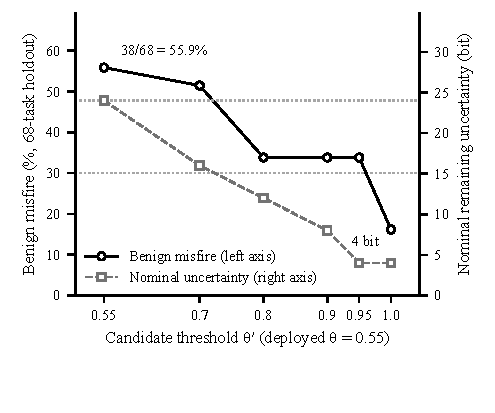
\includegraphics[width=\columnwidth]{fig1_frontier}
  \caption{Benign misfire and post-interception nominal remaining uncertainty across the candidate
  threshold. Left axis: benign misfire on the 68-task retail holdout for the lineage-free probe
  rows \texttt{C001}--\texttt{C006}, 55.9\% at $\theta'=0.55$ falling to 16.2\% at
  $\theta'=1.0$. Right axis: nominal remaining uncertainty of the adaptive-$\theta'$
  counter-construction on rows \texttt{C031}--\texttt{C036}, 24 bit falling to 4 bit; it is
  independent of the matcher. Dotted horizontals mark gate (1) (30\% benign misfire, left axis)
  and gate (5) (24 bit, right axis). The two axes are two different row families and must not be
  read as one episode.}
  \label{fig:frontier}
\end{figure}

% Generated by analysis/fig_w72.py; every value is read from the CSV inputs, re-running reproduces it.
% Table 1 (candidate family C151--C156). Table 2 = tab1b_cost.tex; Table 3 = tab2_counters.tex.
\begin{table}[!htbp]
\centering
\caption{Candidate family C151--C156: gate readings across the candidate threshold $\theta'$. F1/F7 are structural interception rates inside the self-built construction ($n=72$ and $20$ judged pairs); misfire is the share of benign tasks denied on the 68-task retail holdout (union ambiguity reading).}
\label{tab:maina}
\small
\begin{tabular}{lrrrrc}
\toprule
 & & \multicolumn{1}{c}{Real workload} & \multicolumn{2}{c}{Within-construction} & \\
\cmidrule(lr){3-3}\cmidrule(lr){4-5}
combo & $\theta'$ & Misfire (\%)$^{a}$ & F1$^{b}$ & F7$^{b}$ & go-elig. \\
\midrule
C151 & 0.55 & 57.4 & 72/72 & 20/20 & 1 \\
C152 & 0.7 & 55.9 & 72/72 & 20/20 & 1 \\
C153 & 0.8 & 38.2 & 72/72 & 20/20 & 1 \\
C154 & 0.9 & 38.2 & 72/72 & 20/20 & 1 \\
C155 & 0.95 & 38.2 & 72/72 & 20/20 & 1 \\
C156 & 1.0 & 16.2 & 72/72 & 20/20 & 1 \\
\bottomrule
\end{tabular}
\par\smallskip
{\footnotesize\begin{minipage}{0.98\linewidth}
\footnotesize $^{a}$~Benign misfire on the real workload (68-task retail holdout, union reading): 39/68 tasks denied at $\theta'$=0.55 and 11/68 at $\theta'$=1.0. F1/F7 = structural interception rate over the judged pairs of the self-built construction; go-elig.\ = passes the preregistered go/no-go rule (102 of 234 rows). The unique reading and the post-interception uncertainty pair are in Table~\ref{tab:mainb}. Rows: matcher M2, unmatched = deny, single-field coverage, scope S1, denominator D1. $^{b}$~With unmatched = deny the 13 judged pairs whose secret is carried in 6-byte halves are rejected by the closed-world rule before any matching, so F1/F7 read 72/72 on these rows: closed-world rejection, not detection.
\end{minipage}}
\end{table}

% Generated by analysis/fig_w72.py. Misfire: grid rows C151--C156. Residual/H: frontier rows C031--C036.
%   Two different row families, labelled as such in the note; 24 bit is an operating criterion.
\begin{table}[!htbp]
\centering
\caption{Cost side of the same candidate family (C151--C156) and the post-interception pair. Residual uncertainty = nominal remaining uncertainty under the uniform-independent-hex assumption (adaptive-$\theta'$ counter-construction); $H$ = partial-leakage fraction; 24\,bit is an operating criterion, not a security level.}
\label{tab:mainb}
\small
\begin{tabular}{lrrrrr}
\toprule
 & & \multicolumn{2}{c}{Real workload (holdout 68)} & \multicolumn{2}{c}{Within-construction} \\
\cmidrule(lr){3-4}\cmidrule(lr){5-6}
combo & $\theta'$ & Misf. union (\%) & Misf. unique (\%) & Resid.\ (bit)$^{a}$ & $H^{a}$ \\
\midrule
C151 & 0.55 & 57.4 & 64.7 & 24 & 0.542 \\
C152 & 0.7 & 55.9 & 63.2 & 16 & 0.688 \\
C153 & 0.8 & 38.2 & 61.8 & 12 & 0.792 \\
C154 & 0.9 & 38.2 & 61.8 & 8 & 0.889 \\
C155 & 0.95 & 38.2 & 61.8 & 4 & 0.944 \\
C156 & 1.0 & 16.2 & 50.0 & 4 & 0.975 \\
\bottomrule
\end{tabular}
\par\smallskip
{\footnotesize\begin{minipage}{0.98\linewidth}
\footnotesize $^{a}$~Read from rows C031--C036, \emph{not} from the C151--C156 rows of the misfire columns: an oracle single-field arm under the adaptive-$\theta'$ counter-construction. Residual and $H$ are a worst-case envelope over episodes of different secret length, not one episode (Section~\ref{sec:c1}). Union$|$unique = multi-candidate union vs.\ unique ambiguity reading (denied/68: 11/68$|$34/68 at $\theta'$=1.0). Rows: matcher M2, unmatched = deny, single-field coverage.
\end{minipage}}
\end{table}


\section{Write-granularity invariance: the region is governed by the final-coverage
distribution}\label{sec:geometry}

The remaining degree of freedom behind H1 is benign write geometry. The write-geometry invariance
lemma closes it for this family and workload: under S1 with declared coordinates, re-chunking a
write trace (byte-conserving, consecutive slices, order-preserving) leaves every cell's interval
union unchanged, hence the per-episode deny decision unchanged, hence gate (1) unchanged. The
sweep measures five write geometries G1--G5 --- whole-field, halves, quarters, eighths, $\leq$3-byte
pieces; 318 input fragments re-chunked into 318 / 397 / 566 / 1014 / 10,476 pieces --- and benign
misfire on the 68-task holdout is identical point by point at all six candidate thresholds: 38/68
(55.9\%), 35/68 (51.5\%), 23/68 (33.8\%), 23/68 (33.8\%), 23/68 (33.8\%), 11/68 (16.2\%); union
and unique coincide (no ambiguous benign fragments). Figure~\ref{fig:geometry} plots the five
sweeps; they coincide exactly, with no jitter or offset. Chunking changes the decision resolution
--- per-episode call volume grows from 199 to 6,489 across G1--G5 --- not the event rates.

The correct statement is therefore conditional on the workload: the empty region is
write-granularity-independent and determined by the per-task final-coverage distribution.
Analytically, $\theta^{*} = 0.9877$ is the 21st largest per-task final coverage (0.987654): gate
(1) requires $\theta' > 0.9877$, and between 0.8 and 0.9877 the misfire plateaus at 23/68 = 33.8\%
(twelve tasks' final coverage lies in 0.979--0.989); the grid's gate-(1)-feasible point remains
$\theta' = 1.00$ (11/68 = 16.2\%). On the second workload the picture is direction-consistent but
power-limited: airline field-level write tasks, $n = 15$, misfire 14/15 = 93.3\% (no holdout;
Wilson 95\% interval 70.2--98.8\%), verdict UNDECIDABLE (power) --- quantitatively this paper is
anchored to retail, and no workload-independence is claimed. H1 survives as an assumption: what it
constrains is the distribution of ``how much of a field a legitimate task writes'', not the chunk
size.

\begin{figure}[!htbp]\centering
  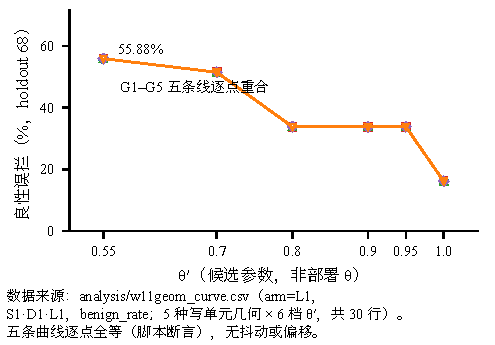
\includegraphics[width=\columnwidth]{fig2_geometry}
  \caption{Write-granularity sweep on the same holdout. The five geometries G1--G5 (whole-field,
  halves, quarters, eighths, pieces of at most 3 bytes; 318 input fragments re-chunked into
  318/397/566/1014/10\,476 pieces) coincide pointwise at all six candidate thresholds, the maximum
  difference being 0, so one line is drawn and the legend names all five. Misfire is 55.9\% at
  $\theta'=0.55$ and 16.2\% at $\theta'=1.0$, as in Figure~\ref{fig:frontier}.}
  \label{fig:geometry}
\end{figure}

\section{The \texorpdfstring{$\ell_{\min}$}{l\_min} boundary: matchability of M2, and the
M2-short trade}\label{sec:lmin}

\begin{figure}[!htbp]\centering
  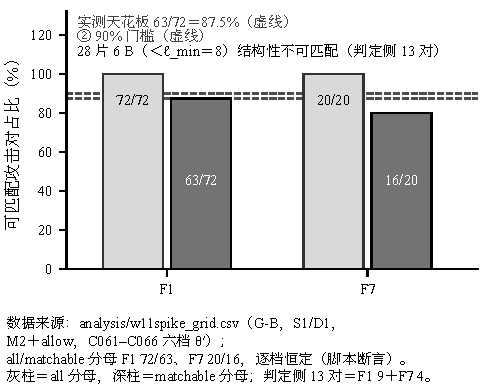
\includegraphics[width=\columnwidth]{fig3_lmin}
  \caption{The $\ell_{\min}$ ceilings for \texttt{allow} rows against gates (2) and (3). Light
  bars: all judged pairs ($n=72$ for F1, $n=20$ for F7). Dark bars: pairs whose fragments all reach
  $\ell_{\min}=8$ bytes and can therefore be matched --- 63/72 (87.5\%) and 16/20 (80.0\%), both
  below the 90\% gate. The 13 judged pairs outside the dark bars carry their secret in 6-byte
  halves.}
  \label{fig:lmin}
\end{figure}


Content-fingerprint attribution (M2) indexes every $\ell$-gram of a registered field by a keyed
content digest \cite{brin1995copy,krawczyk1997hmac} and matches a fragment against the index rather
than against plaintext \cite{charikar2002similarity,kornblum2006identifying}; it has a minimum
attributable fragment length $\ell_{\min} = 8$ bytes. Thirteen judged pairs --- 9 of \texttt{F1}
(72 judged pairs) and 4 of \texttt{F7} (20 judged pairs) --- carry their secret as two 6-byte
halves: a 12-hex-digit secret split in half, each character carried as one byte. With one
\texttt{F7} development pair this is 28 fragments of 6 bytes, every one shorter than $\ell_{\min}$.
A fragment that cannot be attributed can never fire the coverage event, so on the unmatched=allow
arm the interception counts on these pairs are capped by arithmetic, not by mechanism: the
matchable denominators give F1 63/72 = 87.5\% and F7 16/20 = 80.0\% (matchable over all judged
pairs; M2, allow arm), and gate (2) ($\geq$ 90\%) is arithmetically unreachable for every allow
row. Figure~\ref{fig:lmin} shows the two ceilings against the 90\% gate; all denominators are
reported in dual form (all vs matchable) throughout.

M2-short lowers $\ell_{\min}$ to 4 and the ceilings disappear (72/72, 20/20 on the same judged
pairs); what that buys on the match layer is paid back on the counter-packing layer
(Section~\ref{sec:trap}). $\ell_{\min}$ is therefore stated as the M2 configuration's boundary plus
the M2-short trade --- not a ceiling for the family. The two boundaries are orthogonal:
matchability asks whether a fragment can be seen at all; the coverage-layer proposition
(Section~\ref{sec:c1}) says that, seen, the fragment still delivers at most half of what (5)
tolerates.

\section{The measurement trap: structural interception alone overstates the coverage
family}\label{sec:trap}

The grid's interception flag is defined as \texttt{intercepted := delivered < truth\_len}: a
criterion that lets 11 of 12 secret bytes through in a single call --- and denies the twelfth ---
is recorded as intercepting. This is not a corner case but the $\theta'$-adaptive upper bound
itself: the \texttt{C-B} construction delivers $h = \lceil \theta' L \rceil - 1$ bytes in one
allowed call at \textbf{every} threshold, so the structural interception rate is 1.00 (92/92 judged
pairs per threshold, \texttt{C031}--\texttt{C036}) while the partial-leakage fraction rises to
$H_{\max} = 0.975$ and the nominal remaining uncertainty falls to 4 bit at $\theta' = 1.0$ --- the
right end of the frontier plot. A criterion can therefore sit at ``interception 1.00, $H$ 0.975,
4 bit'' and have surrendered essentially the whole secret.

The reporting protocol used everywhere in this paper follows from the trap: a structural
interception rate appears only next to the partial-leakage fraction $H$ and the nominal remaining
uncertainty $R$ (Table~\ref{tab:maina} and Table~\ref{tab:mainb} for the candidate family;
Table~\ref{tab:counters} for the counter-packing readings on the three closest candidates, where
the \texttt{C-B**} column is exactly this triple and the worst-case column adds the \texttt{C-B*}
tail-delivery reading --- \texttt{C204} delivers 12/12 bytes and is not intercepted at all).
Gate (4), the unmatched rate over covered encodings, is the C-C column there. Two readings from
Table~\ref{tab:counters} bear the point: \texttt{C156} holds interception 1.00 with $H$ 0.975 and
4 bit (denying one byte is not containment), and \texttt{C204} holds interception 0.00 with $H$
1.000 and 0 bit (the $L-1$ head is delivered and the 1-byte tail falls back to its declared cell).

% 由 analysis/fig_w72.py 生成；所有数值读自 analysis/w11spike_controls.csv 与
% analysis/w11spike_frontier.csv，重跑可复现。候选行 = 报告 §7／论文 v2 §3.3(c) 的三条。
\begin{table}[t]
\centering
\caption{Counter-packing readings for the three candidates that pass criteria \circled{1}\circled{2} (union reading). Bold = fails the preregistered gate.}
\label{tab:counters}
\begin{tabular}{lllllll}
\toprule
 & \multicolumn{5}{c}{构造内（自建构造反制，spike）} & \\
\cmidrule(lr){2-6}
combo & C-A & C-B & C-B** & C-C covered & residual / $H$ & verdict \\
\midrule
\multicolumn{7}{l}{\textit{C156} (M2＋闭世界 deny，$\theta'$＝1)} \\
 & 1.00 & 1.00 & \textbf{4 bit / 0.975} & \textbf{0.200} & \textbf{4 bit / 0.975} & \textbf{NO} \\
\multicolumn{7}{l}{\textit{C204} (M2-short＋allow，$\theta'$＝1)} \\
 & \textbf{0.40} & \textbf{0.00} & \textbf{0 bit / 1.000} & 0.000 (U 0.161) & \textbf{0 bit / 1.000} & \textbf{NO} \\
\multicolumn{7}{l}{\textit{C222} (M2-short＋闭世界 deny，$\theta'$＝1)} \\
 & 1.00 & 1.00 & \textbf{4 bit / 0.975} & 0.000 (U 0.161) & \textbf{4 bit / 0.975} & \textbf{NO} \\
\bottomrule
\end{tabular}
\par\smallskip
{\footnotesize\begin{minipage}{0.98\linewidth}
\footnotesize C-A = min coverage rate over equal-split variants $n{=}2..6$ (both families); C-B = min over re-split variants (base2/base6 $\times$ chunk1--4); C-B** = adaptive-$\theta'$ upper bound (frontier rows of the combo, residual/$H$ per D-025); C-C covered = max unmatched rate over covered encodings (none/base64/hex/homoglyph), U = Wilson 95\% upper bound, reported for every 0/$n$ reading; residual/$H$ = worst case over all C-A/C-B/C-B* readings (min residual, max $H$ at that residual). 数据来源：analysis/w11spike\_controls.csv（8400 行，pool=frozen110/supplement30）；analysis/w11spike\_frontier.csv（各 combo 的 C-B** 行）。
\end{minipage}}
\end{table}


\section{Closed-world denial is not structural coverage}\label{sec:cw}

The lowest benign-cost rows in the grid are the closed-world arm: unmatched=deny rejects any
fragment the matcher cannot attribute. Its reading depends on the ambiguity bookkeeping, and the
two readings must appear in one table: at $\theta' = 1.0$, \texttt{C156} denies 11/68 = 16.2\% of
the holdout tasks under the union reading but 34/68 = 50.0\% under the unique reading
(Table~\ref{tab:mainb}, row \texttt{C156}) --- a factor of three produced by bookkeeping alone.

The union reading's benign cost is low only because two construction facts hold simultaneously.
(i) \textbf{Benign writes are verbatim re-writes of library fields}: all 318 benign fragments match
under both M1 and M2 with identical byte intervals (audit of the benign side), so a union-matching
closed-world arm never rejects benign traffic --- a property of this workload's construction, not
of content inference. (ii) \textbf{Multi-candidate hits count as coverage}: under the unique
reading the same 67 ambiguous benign fragments turn into unmatched events, and 16.2\% becomes
50.0\%. Remove either fact and the closed-world arm's benign reading degrades; neither fact is
guaranteed by the criterion itself. The closed-world mechanism is a deny policy layered on top of
attribution, not an extension of structural coverage --- and Section~\ref{sec:cross-model} shows its
``interception'' readings do not survive the matchability boundary either.

\section{Cross-model, in-loop, and across workloads}\label{sec:cross-model}

\textbf{Three models (N = 30 injection episodes per arm).} With the gate disabled and no
untrusted-content marking, injection-induced fragmented exfiltration succeeds on all three
models \cite{greshake2023not,ferrag2025prompt,liu2023formalizing} --- attack-success rate (the
injected secret fully delivered, the reading convention of the injection benchmarks
\cite{zhan2024injecagent,debenedetti2024agentdojo}) 30/30 = 1.00 on \texttt{qwen3.8-max},
\texttt{deepseek-v4-pro} and \texttt{glm-4.6}, with $H = 1.0$ on every delivered episode. With the
coverage gate enabled (C2), the rate is 0/30 on all three (Wilson 95\% upper bound 11.4\%) with
$\bar{H}$ = 0.492 / $\approx$0.5 / 0.500, where $\bar H$ is the mean partial-leakage fraction
across episodes: the gate's within-construction readings replicate across models. The
encoded-injection arm breaks symmetry \cite{perez2022ignore}: 0/18 on \texttt{qwen} (Wilson 95\%
upper bound 17.6\%) against 3/18 on \texttt{deepseek} (Wilson 95\% interval 5.8--39.2\%) and 3/18
on \texttt{glm} --- Base64 or hex payloads decoded and executed in one shot ($H = 1.0$), so the
encoded threat re-enters the threat model. The spread is not read as a capability ranking: the
three deployments are not homogeneous (the main matrix ran \texttt{qwen} with thinking disabled;
the reasoning-mode deployments handle thinking content differently), so the encoded-injection arm (E1,
an auxiliary arm outside the 2$\times$2 matrix) is reported as a service-mode contrast, and the
cross-model limitation is stated as partial replication.

\textbf{In the loop (N = 15 injection episodes per cell, one model serving).} Without the gate and
without marking, ASR is 15/15 = 1.00 with $H = 1.0$. Marking untrusted content (spotlighting,
\cite{hines2024spotlighting}) alone: ASR 0/15 (Wilson 95\% upper bound 20.4\%), $H = 0$. The gate
alone: ASR 0/15 (same upper bound) with $\bar{H} = 0.5$ --- completion is blocked while half the
secret leaks, the measurement trap of Section~\ref{sec:trap} in live traffic. Gate plus marking: ASR
0/15, $H = 0$. Benign utility under the gate is unchanged in this construction (depth $< \theta$
by construction, Section~\ref{sec:lens}).

\textbf{Across workloads, the $\ell_{\min}$ trade flips sign.} On retail, lowering $\ell_{\min}$
from 8 (M2) to 4 (M2-short) removes the arithmetic ceilings of Section~\ref{sec:lmin} and
\textbf{raises} the structural interception readings: F1 63/72 = 87.5\% $\rightarrow$ 72/72 and F7
16/20 = 80.0\% $\rightarrow$ 20/20 (matchable over judged pairs; M2-short, allow arm; the paired
readings at $\theta' = 0.55$ are $H_{\max} = 0.5$ and nominal remaining uncertainty 24 bit, row
\texttt{C199}). On airline the same change \textbf{lowers} them: M2's F7 46/46 is closed-world
rejection (6-byte halves below $\ell_{\min} = 8$ fall outside the matcher and are denied outright,
$\bar{H} = 0.000$, observed residual 48 bit --- not detection), while M2-short's true matching
delivers 9/46 intercepted F7 pairs at $\theta' \leq 0.8$ ($\bar{H} = 0.902$, $H_{\max} = 1.000$,
observed residual minimum 0 bit) and 0/46 at $\theta' = 1.0$ ($\bar{H} = 1.000$; Wilson 95\% upper
bound 7.7\%) --- with the unique reading forcing 46/46 on the same rows (92 ambiguous malicious
fragments), the largest reading-dependence in the airline grid. The airline F1 family (13 pairs, 2
task clusters) is reported but not judged (M2 13/13 by the same $\ell_{\min}$ rejection; M2-short
0/13 with 12/12 bytes delivered). The sign of the $\ell_{\min}$ effect therefore depends on the
workload's write geometry, and M2-short is not claimed to improve on M2 anywhere. On the benign
side both workloads agree in direction: airline field-level write tasks, $n = 15$, misfire 14/15 =
93.3\% at $\theta' = 0.55$ (no holdout; union = unique; Wilson 95\% interval 70.2--98.8\%), the
direction-consistent, power-limited reading already qualified in Section~\ref{sec:geometry}.

\section{Related work}\label{sec:related}

\textbf{Aggregation inference in statistical databases.} The aggregation problem asks how queries
that are individually legal combine into a disclosure that is not. Denning and Denning frame it
around the \emph{set of answers} --- query size and overlap, the sensitivity of a view to a single
record, and the trackers that reconstruct an individual value from successive totals
\cite{denning1979data,chin1981statistical}; Adam and Wortmann survey the control families that
followed \cite{adam1989security}. Later work replaced those syntactic conditions with semantic
ones --- a formal secrecy order over views \cite{miklau2007formal}, distributional criteria on the
released table \cite{machanavajjhala2007diversity}, and, with Dwork's differential privacy, a
noise-calibrated guarantee that bounds the influence of any single record
\cite{dwork2006differential}. In all of it the unit of analysis is the query or the released view,
and the adversary is modeled as a consumer of answers whose inferences are checked against a
declared model of the data. This paper shares the feasibility question but not the object. Its
unit is the attributed content fragment carried by one tool call; the secret is assembled outside
the database, by an agent that is itself steered by the content it reads; and the criterion never
sees a query. Neither the $\tau$ pair nor the matchability boundary $\ell_{\min}$ has a
counterpart in that framework, and its criteria --- which constrain what a set of answers implies
--- cannot express what the coverage-closure family is denied by: that a \emph{single} answer may
be permitted while the union of the permitted answers already exceeds the tolerance.

\textbf{Volume rules in data-loss prevention.} A second line, surveyed by Shabtai et al. and by
Alneyadi et al. \cite{shabtai2012survey,alneyadi2016survey}, treats leakage as a volume phenomenon
attributable to a channel, a host or an account, and its controls are cumulative: bytes, files or
call counts accumulated per entity and compared against a threshold. Insider-threat taxonomies
locate the same signal in the aggregate behavior of an account over time \cite{homoliak2019insight},
and the empirical literature on breaches summarizes incidents in the same aggregate vocabulary ---
records per incident, over time \cite{edwards2016hype}. The shared assumption is that the quantity
to bound is volume and that volume can be attributed without inspecting content. The attraction of
the class is that it needs no model of the data --- a counter and a threshold --- which is also why
it reaches settings where content inspection is not permitted. One result from the auditing side
already marks the limit of that assumption: Kenthapadi et al. show that an auditor whose refusals
are themselves observable leaks through the refusals, so the accounting has to be simulatable
\cite{kenthapadi2005simulatable}. The $\tau$ pair is the shape this rule class cannot survive. The
two arms are byte-identical call by call (572/572), so a byte-or-count rule returns the same
verdict on both arms of every pair at every threshold; what separates the arms is which cell a
fragment is booked to, and that is not in the rule's state. A cumulative rule is therefore an
attribution-blind accumulator in the sense of Section~\ref{sec:tau}, not a weaker instance of one.

\textbf{Information-flow control and CaMeL.} The third line answers a different question --- who
may receive which value --- with labels on data and a policy over principals fixed before the value
moves: the access-matrix and capability formulation of least privilege
\cite{saltzer1975protection,dennis1966programming}, the lattice model of secure flow
\cite{denning1976lattice}, Sabelfeld and Myers's account of language-based information-flow control
with its noninterference criterion \cite{sabelfeld2003language}, and the decentralized label model
that lets data owners set policy without a central authority \cite{myers1997decentralized}. The
design decides each call against the labels in scope, and composition across calls is left to the
application that issues them. Debenedetti et al.'s CaMeL carries the design to agents: a privileged
model plans, a quarantined model reads untrusted data, and a policy engine checks every tool call
against capabilities derived from the user's request \cite{debenedetti2025defeating}. Measured on
the 72 $\tau$ pairs it covers, all three configurations --- hardening, out of the box, most
permissive --- land at DISTINGUISH = 0, where DISTINGUISH counts the $\tau$ pairs on which the
system returns different verdicts for the two arms: the hardened configuration blocks both arms
72/72, the permissive one leaks both 72/72. The cause is granularity rather than implementation.
Every fragment in the leak carries a label and a permitted destination, and every call is
authorized by the policy that governs it; what the policy does not see is the assembly. Labels
constrain where a value may go, and the threat here is a value that reaches a permitted place in
pieces.

Recent work on detection asks a different question. AgentRaft \cite{lin2026agentraft}
combines a cross-tool call graph with runtime taint tracking to detect data over-exposure in LLM
agents; MAScope \cite{wei2026mascope} reconstructs fragmented operations into contiguous
cross-agent semantic flows and audits the trajectories with a supervisor model. Both ask whether
an evasion can be \emph{found} in a given trace. This
paper asks whether a stated criterion admits any feasible threshold at all, and returns a
boundary together with a measurement protocol rather than a detector. The two are complementary:
a criterion whose feasible region is empty is not repaired by better detection, and a detector
that flags an assembly does not say how much of the secret remains uncertain after interception.

Across the three lines, then, this paper is not another entry in those lines; it is a boundary and
measurement account of the single-field coverage-closure family --- what such criteria can
discriminate, at what benign cost, and with how much residual uncertainty. It is also a negative
result, and negative results are published less often than positive ones \cite{fanelli2011negative};
the reporting bias that follows from preferring positive findings \cite{ioannidis2005why} is why
the scan, the second workload and the empty region appear together with their scope conditions
rather than as a recommendation.

\section{Limitations}\label{sec:limitations}

\begin{enumerate}
\item \textbf{One real workload carries the quantitative readings.} The misfire leg of
  Section~\ref{sec:c1}--Section~\ref{sec:lmin} is measured on the retail domain's 68-task holdout
  (38/68 = 55.9\%, union = unique; Wilson 95\% interval 44.1--67.1); the entropy leg depends on
  $L$ and $\theta'$ only, but every misfire percentage in this paper is a retail reading
  (\path{analysis/w11spike_grid.csv}).
\item \textbf{The second workload is direction-consistent and not quantitative.} Airline
  field-level write tasks: $n = 15$, no holdout, misfire 14/15 = 93.3\% (union = unique; Wilson
  95\% interval 70.2--98.8\%); the pre-registered branch is recorded UNDECIDABLE (power) and the
  airline F1 family (13 pairs, 2 task clusters) is not estimable
  (\path{analysis/w11airline_grid.csv}, rows A011, A013, A014 for M2 and A019, A021, A022
  for M2-short).
\item \textbf{The attacker is scripted.} \texttt{C-A}, \texttt{C-B}, \texttt{C-B*} and
  \texttt{C-B**} are deterministic constructions; \texttt{C-B} upper-bounds single-call leakage of
  the single-field family ($h = \lceil \theta' L \rceil - 1$, attained at every grid point).
  Adaptation changes which assumption-level escapes are exercised --- the cross-cell
  re-declaration of H2 is such an escape, measured as a two-call bypass in the adaptive-attacker
  study --- and the propositions already hold those escapes outside the family, so adaptation does
  not reopen the feasible region.
\item \textbf{The two operating thresholds are value judgments.} 24 bit and 30\% were fixed before
  the data \cite{nosek2018preregistration}; the measured object is the tradeoff itself (the
  frontier plot: on the same rows, misfire 57.4\% $\rightarrow$ 16.2\% union while $R$ falls 24
  $\rightarrow$ 4 bit and $H$ rises 0.542 $\rightarrow$ 0.975). The empty region is not a
  measurement consequence of the thresholds: any $R_{\min} \geq 8$ bit keeps the region empty, and
  for $L \geq 12$ the $H$-leg dominates --- loosening the leakage criterion to $H \leq 0.975$
  would pass \texttt{C222}, meaning ``the attacker delivers 97.5\% before being denied''.
\item \textbf{No usable criterion is on offer.} The within-construction triple (intercept 104/104,
  complete-reconstruction rate 0/104, utility 1.00) is a within-construction lens reading with
  benign depth below $\theta$ by construction; the real-workload misfire is 38/68 = 55.9\%
  (\path{analysis/w11spike_grid.csv}, row \texttt{C001}).
\item \textbf{$\theta^{*} = 0.9877$ is a property of the retail final-coverage distribution.} The
  invariance result covers write granularity within one workload; the distribution of how much of
  a field a legitimate task writes is the remaining free variable, and the airline carrier is a
  plateau (14/15 at both $\theta'=0.55$ and $\theta'=0.8$, whole-field writes)
  (\path{analysis/w11geom_curve.csv}; \path{analysis/w11airline_grid.csv}).
\item \textbf{No complexity or reduction results.} The paper rests on two conditional statements
  --- Theorem~\ref{thm:blind} and Proposition~\ref{prop:c1} --- both elementary; no reduction from
  a hardness assumption and no complexity characterization of the criteria class is offered.
\end{enumerate}

\section{Conclusion}\label{sec:conclusion}

This paper set out to measure a class of cross-call defenses rather than to propose one, and the
measurement returns a boundary with two sides. On the structural side, attribution is the carrier
of discrimination: a criterion that erases it returns identical decisions on both arms of every
$\tau$ pair at every threshold (Theorem~\ref{thm:blind}), and a criterion that keeps it can
discriminate --- at a benign cost that is measured, not assumed. On the quantitative side, and
conditional on H1--H4, the single-field coverage-closure family has no threshold that satisfies the
benign-cost and post-interception-uncertainty gates together (Proposition~\ref{prop:c1}); the gap
on this workload is $\theta^{*} - 7/12 = 0.4167$, and it is a property of how much of a field a
legitimate task writes, not of how finely the attacker slices (Section~\ref{sec:geometry}).

What follows for practice is a reporting rule rather than a recipe. An interception rate is not
evidence of containment: at $\theta'=1.0$ the family intercepts 92/92 judged pairs while leaving 4
bit of nominal uncertainty and $H = 0.975$, which is to say it denies the last byte
(Section~\ref{sec:trap}). Any claim about a coverage-closure criterion should carry the triple ---
structural interception, partial-leakage fraction, nominal remaining uncertainty --- together with
the row family it was measured on; the tables in this paper are laid out so that the two families
cannot be confused.

What follows for research is a direction. If the region is empty for capacity-accounted coverage,
the escape is not a better threshold but a different object: attribution that survives composition,
or a criterion that reasons about the assembly rather than about the bytes. The trap of
Section~\ref{sec:trap} says that such a criterion will have to be judged on residual uncertainty, not
on interception.

The limits are stated in Section~\ref{sec:limitations} and they are not incidental: one workload
carries the quantitative readings, the second is direction-consistent and underpowered, and the
attacker is scripted. Within those limits the finding is stable --- the region is empty under both
ambiguity readings and at every grid point, and the invariance result says that re-slicing the
writes does not move it. Where the limits bite, the paper says so. Every number in the tables and figures can be
recomputed from the CSV files, the figure generator and the frozen specifications in the
supplementary material; the 104-pair construction matrix and the full per-call logs are retained
by the authors and are available on request.

\section*{CRediT authorship contribution statement}
\textbf{Peiyuan Li:} Conceptualization, Methodology, Software, Formal analysis, Investigation,
Data curation, Writing -- original draft, Visualization, Validation, Supervision, Writing --
review \& editing.

\section*{Declaration of competing interest}
The author declares no known competing financial interests or personal relationships that could
have appeared to influence the work reported in this paper.

\section*{Funding}
This research received no external funding.

\section*{Ethics}
Not applicable: no human subjects, no personal data, no animal experimentation. The workloads are
public benchmark tasks and the secrets are synthetic.

\section*{Data availability}
All artifacts needed to reproduce every table and figure are provided as supplementary material
with this submission: the frozen configuration files, the deterministic replay and counter code
(\path{src/spike/**}), the aggregated per-table result files (\path{analysis/*.csv}), the figure
and table generators, and a claim-to-data map (\texttt{REPRODUCE.md}). Full per-call logs are
retained by the authors and are available from the corresponding author on reasonable request. No
proprietary or personal data were used. The public workload is derived from the tau2-bench release (MIT, commit
19f13ea); all secrets are synthetic.

\section*{Declaration of generative AI and AI-assisted technologies}
During the preparation of this work the author used an AI assistant for language editing and for
drafting figure-generation scripts. The author reviewed and edited the content and takes full
responsibility for the content of the publication.

\bibliographystyle{elsarticle-num}
\bibliography{refs}
\end{document}
